\documentclass{article}

% Language setting
% Replace `english' with e.g. `spanish' to change the document language
\usepackage[english]{babel}

% Set page size and margins
% Replace `letterpaper' with `a4paper' for UK/EU standard size
\usepackage[letterpaper,top=2cm,bottom=2cm,left=3cm,right=3cm,marginparwidth=1.75cm]{geometry}

% Useful packages
\usepackage{amsmath}
\usepackage{graphicx}
\usepackage[colorlinks=true, allcolors=blue]{hyperref}
\usepackage{listings}
\lstset{language=R,
    basicstyle=\small\ttfamily,
    stringstyle=\color{DarkGreen},
    deletekeywords={I, df, aov},
    keywordstyle=\color{blue},
    commentstyle=\color{DarkGreen},
    numbersep=8pt
}
\usepackage{enumitem}
\renewcommand\thesubsection{\Alph{subsection}}

\title{Report 1}
\author{You}

\begin{document}
\maketitle

\begin{abstract}
Your abstract.
\end{abstract}

\section{Ice cream}


\section{Hemoglobin in trout}

\begin{figure}[h]
    \centering
    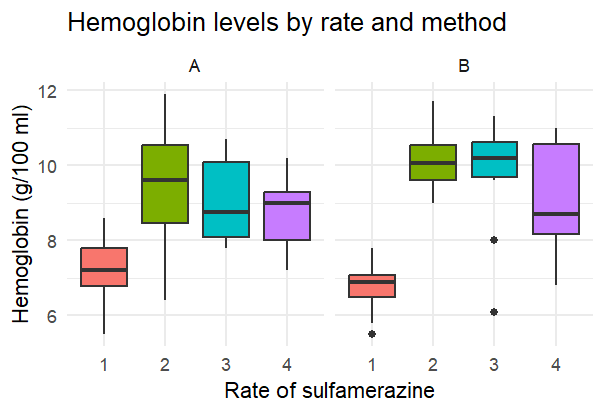
\includegraphics[height=5cm]{BoxplotHemoglobin.png}
    \caption{This boxplot illustrates the variation of hemoglobin levels across different rates of sulfamerazine, categorized by two different methods (A and B). Rates are defined as 0, 5, 10 and 15 grams of sulfamerazine per 100 pounds of fish. The rate of 1, indicating no sulfamerazine, is associated with lower hemoglobin levels compared to higher rates. }
    \label{fig:boxHem}
\end{figure}

\subsection{Randomization in R}
This dataset has an numerical data for hemoglobin and two factors (rate and method) that have levels (1,2,3,4 for rate, A and B for method). This dataset has a balanced design, because every combination of rate and method has 10 observations (N). This can be denoted as $n_{i,j} = N$, for subgroups rate (i) and method (j).
\begin{lstlisting}[caption="Randomization in R",label={lst:R}]
    rbind(rep(1:I, each = N * J), rep(1:J, N*I), sample(1:(N*I*J)))
\end{lstlisting}
in Listing \ref{lst:R}, an R-code for the randomization process to distribute 80 fishes over all combinations of levels of factors rate and method is shown.

\subsection{Two-way ANOVA}
To test the effects of factors rate, method and their interaction on the response variable hemoglobin, a Two-way ANOVA test was performed following the R-code in Listing \ref{lst:T}. 
\begin{lstlisting}[caption="Two-way ANOVA", label={lst:T}]
    hemoglobin_df$rate <- as.factor(hemoglobin_df$rate) 
    hemoglobin_df$method <- as.factor(hemoglobin_df$method)
    hemoglobin_aov <- lm(hemoglobin ~ rate*method, data = hemoglobin_df)
    anova(hemoglobin_aov)   
\end{lstlisting}
rate * method indicates rate + method + rate:method, so in this test, we test if interaction can be disregarded. 

\begin{table}[ht]
\centering
\caption{Two-way ANOVA Table for Hemoglobin Levels by Rate and Method} 
\label{tab:hemoglobin_anova}
\begin{tabular}{lrrrrr}
  \hline
 & Df & Sum Sq & Mean Sq & F value & Pr($>$F) \\ 
  \hline
rate & 3 & 90.56 & 30.19 & 19.47 & 0.0000 \\ 
  method & 1 & 2.42 & 2.42 & 1.56 & 0.2161 \\ 
  rate:method & 3 & 4.87 & 1.62 & 1.05 & 0.3769 \\ 
  Residuals & 72 & 111.64 & 1.55 &  &  \\ 
   \hline
\end{tabular}
\end{table}

The p value for testing H0: $\gamma_{i*j}$ = 0 for all (i, j) is 0.3769. which means there is no evidence for interaction. We do not reject the hypothesis, so we can use the additive model to test which factor has most effect on the hemoglobin levels. 

\begin{table}[ht]
\caption{Treatment Parameterization in ANOVA}
\label{tab:treatment}
\centering
\begin{tabular}{rrrrr}
  \hline
 & Estimate & Std. Error & t value & Pr($>$$|$t$|$) \\ 
  \hline
(Intercept) & 7.2000 & 0.3938 & 18.28 & 0.0000 \\ 
  rate2 & 2.1300 & 0.5569 & 3.82 & 0.0003 \\ 
  rate3 & 1.8300 & 0.5569 & 3.29 & 0.0016 \\ 
  rate4 & 1.4900 & 0.5569 & 2.68 & 0.0092 \\ 
  methodB & -0.4500 & 0.5569 & -0.81 & 0.4217 \\ 
  rate2:methodB & 1.2600 & 0.7875 & 1.60 & 0.1140 \\ 
  rate3:methodB & 1.1500 & 0.7875 & 1.46 & 0.1486 \\ 
  rate4:methodB & 0.7800 & 0.7875 & 0.99 & 0.3253 \\ 
   \hline
\end{tabular}
\end{table}

\subsection{Additive model}
\begin{lstlisting}[caption="Additive model for Two-Way ANOVA", label={lst:Add}]
    hemoglobin_aov_2 <- lm(hemoglobin ~ rate+method, data = hemoglobin_df)
    anova(hemoglobin_aov_2) 
\end{lstlisting}


\subsection{One-way ANOVA}

\subsection{Kruskal-Wallis test}


\section{Exercise 3}


\bibliographystyle{alpha}
\bibliography{sample}

\end{document}